% !TEX root = ../../Diploma.tex
\section{Learning a New Behaviour}
\subsection{Training with a long episode and high discount factor}
Since it could be shown, that the agent can improve the static parameters of a control strategy, the next step is to attempt to train an agent to learn a new behaviour. As described in \ref{ssec:new_behaviour_description}, three agents controlling the generator torque of the three turbines are trained. First, an agent with a long episode and a high discount factor will be examined. The long episode is chosen to allow the agent to develop lower frequency strategies. As was noted in \autoref{ssec:new_behaviour_description}, a high discount factor is chosen from an analysis of the physical timescales of the wind park.
\begin{figure}[h]
	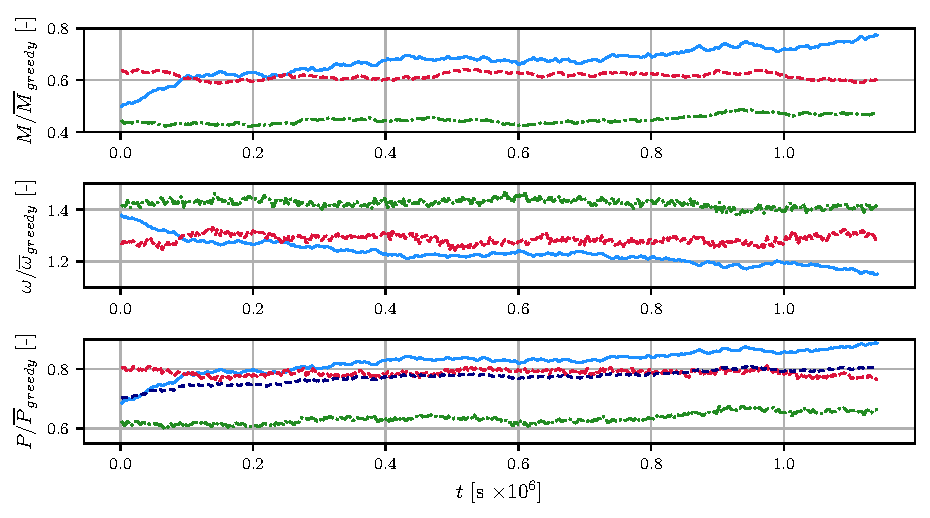
\includegraphics{plots/behaviour_optimization/torque_long_high_training.pdf}
	\caption{\legendFour{Turbine 0}{Turbine 1}{Turbine 2}{Total} Training of agent with $\gamma=0.99$ and for episodes with $N_{a,e}=1500$.}
	\label{fig:torque_long_high_training}
\end{figure}\\
The timeseries of the generator torques, the angular velocities and the generated power of the three turbines as well as the total generated power are shown in \autoref{fig:torque_long_high_training}. It shows that after $\SI{1.2e6}{s}$ the performance by the agent is still significantly worse than that of a greedy controller. Therefore the training was stopped at this point. Furthermore, only minor improvement in total power is visible for $\SI{1e5}{s}$. The figure shows, that the torque of the first turbine is steadily increased throughout the training, while the torque of the second and third turbine show little change.
\begin{figure}[h]
	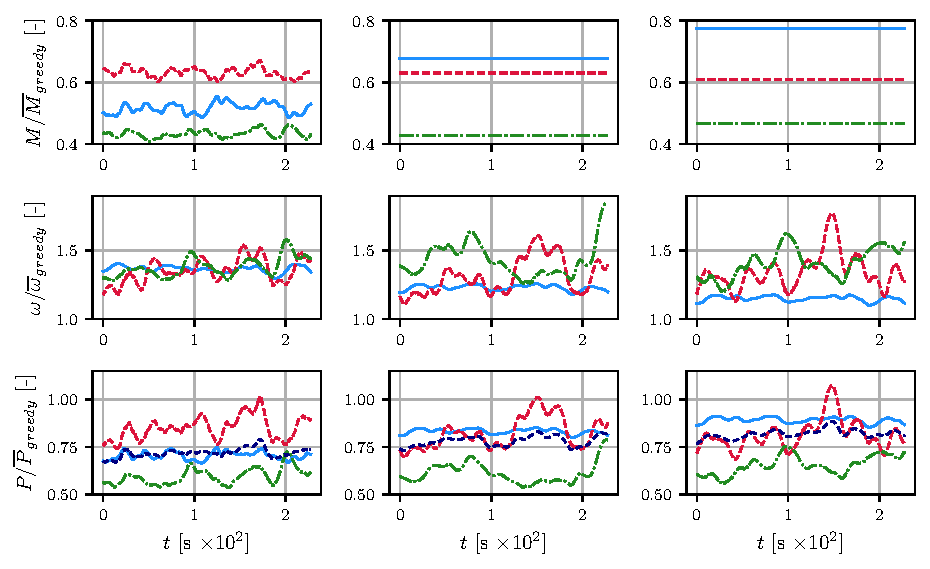
\includegraphics{plots/behaviour_optimization/torque_long_high_eval.pdf}
	\caption{\legendFour{Turbine 0}{Turbine 1}{Turbine 2}{Total.}Evolution of control strategy of agent with $\gamma=0.99$ and for episodes with $N_{a,e}=1500$. Left column is control strategy in the beginning of training, central column after half of the training and right column after training has finished.}
	\label{fig:torque_long_high_eval}
\end{figure} \\
To analyze the evolution of the control strategy, despite it not being successful, \autoref{fig:torque_long_high_eval} shows generator torque, angular velocity and generated power by the turbines when controlled by the agent after 12 updates, after half of training time and after the full training time. The comparison of the control strategies shows that the agent evolves to set a constant generator torque at all three turbines. This is already visible after half of the training time. Furthermore, as was seen in \autoref{fig:torque_long_high_training}, the generator torque of the first turbine increases, while the torque at the other two turbines does not change significantly after half of the training. Since the power of the first turbine is greatest, it appears reasonable that control of that turbine is improved fastest. A static generator torque differs from greedy control, but considering that the inflow has a uniform mean value, such a strategy can still be reasonable. However, since the total generated power only reached about three quarter of the total power of a greedy-controlled park, this strategy will not be investigated further. The major drawback of this agent was the slow evolution. One of the possible reasons for this is the low number of updates of the agent per simulated time due to long episodes. Furthermore, the reason for the long episode was the ability to develop lower frequency behaviour, which did not occur. Therefore another agent with a shorter episode  was trained. \newpage
\subsection{Training with a short episode and high discount factor}
To increase the number of updates per simulated time, an agent with a number of actions per episode of 500 was trained.  
\begin{figure}[h]
	\centering
	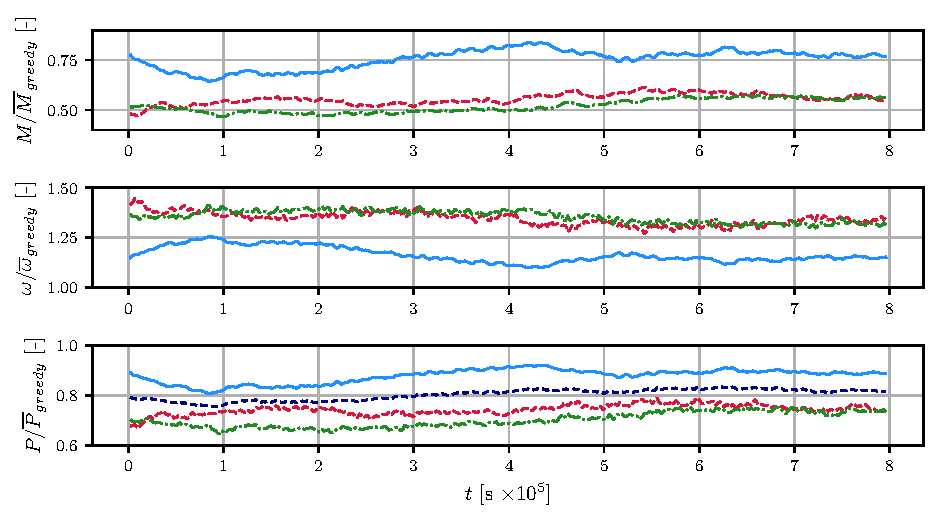
\includegraphics{plots/behaviour_optimization/torque_short_high_training.pdf}
	\caption{\legendFour{Turbine 0}{Turbine 1}{Turbine 2}{Total.}Training of agent with $\gamma=0.99$ and for episodes with $N_{a,e}=500$.}
	\label{fig:torque_short_high_training}
\end{figure}\\
The time series of the generated power, angular velocity and generator torque are shown in \autoref{fig:torque_short_high_training}. It shows that total generated power, after an initial decrease, increased for about half of the training. After that, total power did not increase, but the mean of the controlled variables, the generator torques, still changed. Therefore training was continued further, but the agent returned to the same strategy multiple times. Thus training was stopped after $\SI{8e5}{s}$. The comparison to the previous agent with a longer episode shows, that the behaviour of the agent changes faster. Yet it is not able to develop a strategy that performs as good as a greedy controller. While the first turbine performs almost as good as a single greedy controlled turbine, the second and the third turbine perform considerably worse. The plot also shows that the changes in the control strategy for these two turbines are smaller than the changes in strategy for the first turbine. Again, this can be explained by the larger power produced at the first turbine. 
\begin{figure}[h]
	\centering
	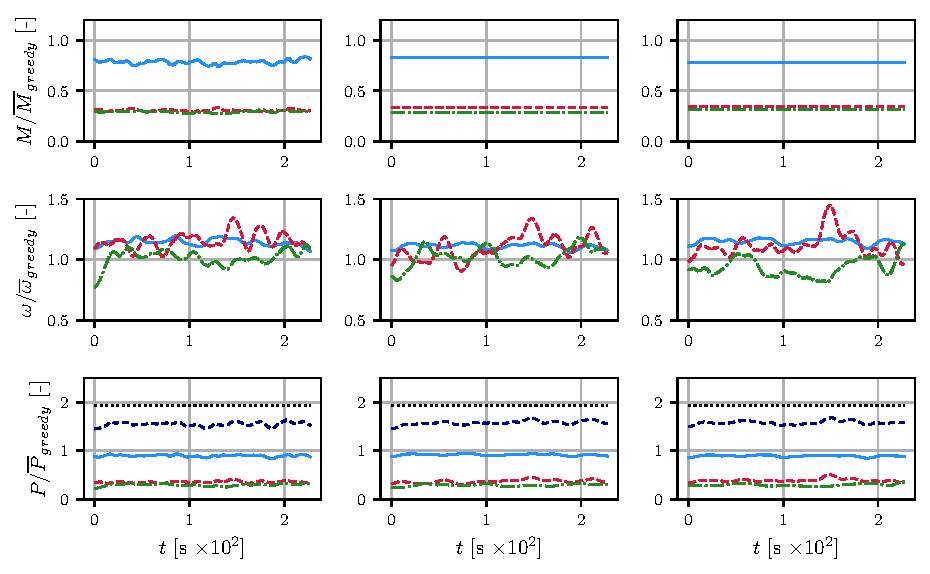
\includegraphics{plots/behaviour_optimization/torque_short_high_eval.pdf}
	\caption{\legendFour{Turbine 0}{Turbine 1}{Turbine 2}{Total.}Evolution of control strategy of agent with $\gamma=0.99$ and for episodes with $N_{a,e}=500$. Left column is control strategy in the beginning of training, central column after half of the training and right column after training has finished.}
	\label{fig:torque_short_high_eval}
\end{figure}
To find out more about the developed strategy and how it changed throughout the training, \autoref{fig:torque_short_high_eval} shows generator torques, angular velocities and generated powers per turbine as well as total generated power for parks controlled by agents at the beginning of the training, after half the training and after training has been completed. It shows that this agent also developed the strategy to set constant generator torques.  It also  shows that the first turbine performs almost as good as a greedy controlled turbine. In comparison to the greedy controller the agent sets a lower generator torque at all of the turbines, therefore they have higher angular velocities. Thus the thrust forces exerted by the turbines are also higher, resulting in a higher wake deficit. Consequentially the downstream turbines perform worse. However it is not clear why the agent does not set higher torques to reduce thrust. As was explained in \autoref{ssec:new_behaviour_description}, the high discount rate leads to consideration of rewards that occur far in the future. This leads to a noisy signal, where influences of later actions also play a role. In combination with a turbulent flow that is by definition noisy, this might inhibit optimization as the correlation between return, which is the discounted sum of total generated power, and generator torque at one point in time is too low to have a significant effect on the agent. To reduce the noise in the signal an agent is trained with a lower discount rate. \newpage
\subsection{Training with a short episode and low discount factor}
A return computed with a discount rate of $\gamma=0.99$ includes the influence of the first turbine on the second. However, this might also lead to the inclusion of too many time steps into the return, thus making it impossible for the agent to improve its behaviour. Therefore an agent with a discount rate of $\gamma=0.95$ was trained as well.
\begin{figure}[h]
	\centering
	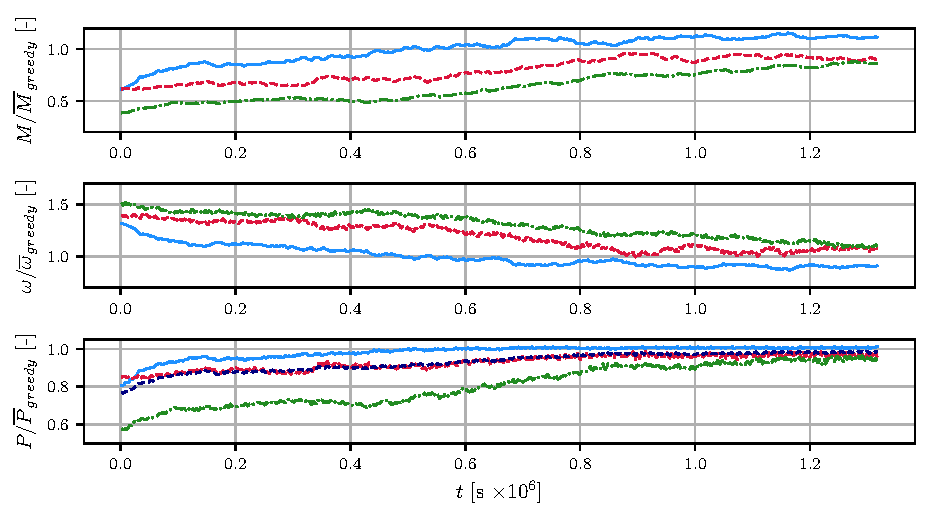
\includegraphics{plots/behaviour_optimization/torque_short_low_training.pdf}
	\caption{\legendFour{Turbine 0}{Turbine 1}{Turbine 2}{Total.}Training of agent with $\gamma=0.95$ and for episodes with $N_{a,e}=500$.}
	\label{fig:torque_short_low_training}
\end{figure} \\
The time series of the training of that agent is shown in \autoref{fig:torque_short_low_training}. This agent did learn a behaviour that performs almost as good as the greedy control. While the gain in total power in the beginning of training can be attributed to an increase in power produced by the first turbine, the third turbine also improves continuously. The second turbine also improves in power with time, although the gains are smaller. The training is conducted for $\SI{1.3e6}{s}$, which is longer than for the previous agents, but the strategy had not finished improving after $\SI{8e5}{s}$. A look at the generator torques shows that the torque at all three turbines increased throughout the training, which in turn lead to a decrease in angular velocity at all three turbines. The overall development of power and torque looks similar to that of the first agent as shown in \autoref{fig:torque_long_high_training}. As length of episode and discount factor both influence the return, both these agents seem to have a good ratio of these factors. As the long episode agent did not develop a dynamic control strategy, the long episode does not offer advantages, but only increases the simulated time per update. 
\begin{figure}[h]
	\centering
	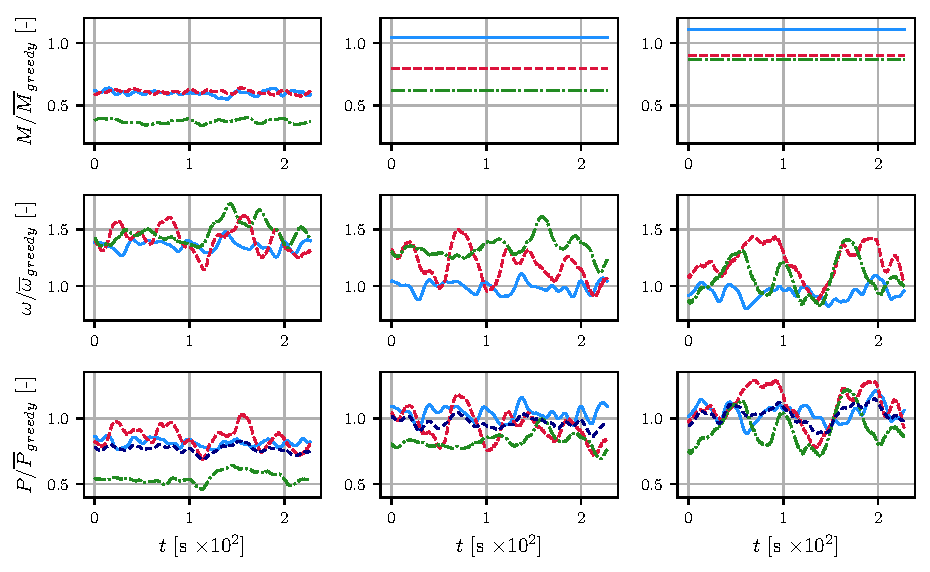
\includegraphics{plots/behaviour_optimization/torque_short_low_eval.pdf}
	\caption{\legendFour{Turbine 0}{Turbine 1}{Turbine 2}{Total.}Evolution of control strategy of agent with $\gamma=0.95$ and for episodes with $N_{a,e}=500$. Left column is control strategy in the beginning of training, central column after half of the training and right column after training has finished.}
	\label{fig:torque_short_low_eval}
\end{figure} \\
The evolution of the strategy is shown in \autoref{fig:torque_short_low_eval}. It shows that this agent, like the other two previously studied, sets a constant generator torque after half of the training and does not react to the flow any more. The strategy in the second half of the training only changes in the constant torque that is set. As was visible in \autoref{fig:torque_short_low_training}, the torques set all increase in value. The final control strategy sets a higher torque at the first turbine than the mean torque set by a greedy controller. Furthermore it shows that, since a constant generator torque is set, angular velocities fluctuate due to the turbulent inflow. Furthermore these fluctuations are also visible in the generated power. As was mentioned in the analysis of the first generator torque controlling agent, one reason for the development of the static strategy might be that the mean inflow velocity is constant and only superimposed with fluctuations. Thus in the mean this strategy is comparable to a very slow greedy controller.
\subsection{Analysis of flow}
\begin{table}[h]
	\centering
	\caption{Mean, relative difference in mean and relative in standard deviation of power and aerodynamic moment of a trained torque-controlling agent in comparison to the greedy-control case.}
	\begin{tabular}{ccccccc}
		\toprule
		& \multicolumn{3}{c}{$P$}  & \multicolumn{3}{c}{$M_{aero}$ }\\ \cmidrule(rl){2-4} \cmidrule(rl){5-7}
		& mean & rel. mean & rel. std  & mean & rel. mean & rel. std \\ \midrule
		Total & $\SI{  9.65}{MW} $ & $\SI{ -1.42}{\%}$ & $\SI{ -19.3}{\%}$ &-&-&- \
		\\
		Turbine 0  & $\SI{   5.1}{MW} $ & $\SI{+0.837}{\%}$ & $\SI{ +6.28}{\%}$ & $\SI{3.53e03}{kNm} $ & $\SI{ +10.6}{\%}$ & $\SI{ +14.8}{\%}$ \\
		Turbine 1  & $\SI{  2.48}{MW} $ & $\SI{ -3.23}{\%}$ & $\SI{ -22.5}{\%}$ & $\SI{1.82e03}{kNm} $ & $\SI{ -9.65}{\%}$ & $\SI{ -4.19}{\%}$ \\
		Turbine 2  & $\SI{  2.07}{MW} $ & $\SI{ -4.55}{\%}$ & $\SI{ -26.1}{\%}$ & $\SI{1.57e03}{kNm} $ & $\SI{ -13.2}{\%}$ & $\SI{ -6.25}{\%}$ \\
		\bottomrule
	\end{tabular}
	\label{tab:torque_quants}
\end{table}
In \autoref{tab:torque_quants} mean values as well as relative changes in mean and standard deviation compared to a greedy controlled case are shown for power and aerodynamic torque. The total power production is $1.42$ percent lower than that of a greedy controlled park. Since the agent has not necessarily converged yet, it is possible that further training would lead to a performance as good as that of the greedy controlled park. In comparison to the greedy controlled park, power produced by the second and third turbine decreased, while first turbine produces negligibly more. But while the primary objective, the increase in total power could not be reached, the quality of overall power significantly improved with a reduction in standard deviation of $19.3$ percent. This is due to a decrease in fluctuations at the second and third turbine, while fluctuations at the first turbine increased. The same is true for the aerodynamic moment. The mean as well as the standard deviation increased at the first turbine while they were considerably reduced at the second and third turbine. As especially power quality is of growing concern, a more thorough analysis of the flow might offer insights into how this reduction is achieved.
\begin{figure}[h]
	\centering
	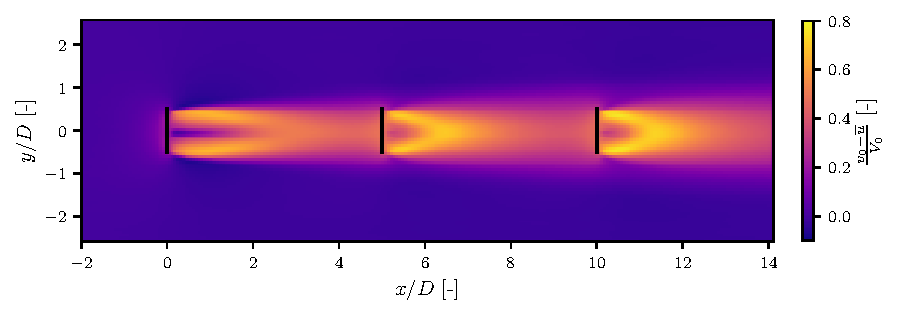
\includegraphics{plots/behaviour_optimization/torque_short_low_velocity.pdf}
	\caption{{\color{black} \rule[3pt]{22pt}{1pt} Turbine.} Mean wake deficit of ANN-controller.}
	\label{fig:torque_vel}
\end{figure} \\
To this end, \autoref{fig:torque_vel} shows the wake deficit in the domain. The deficit is largest in the wake of the third turbine and smallest after the first turbine. In comparison to the results of the helix control, the wake is not as wide. The deficit in front of the second and third turbine is larger, which explains why the generated power controlled by this controller is lower than the power generated by both of the helix controllers. 
\begin{figure}[h]
	\centering
	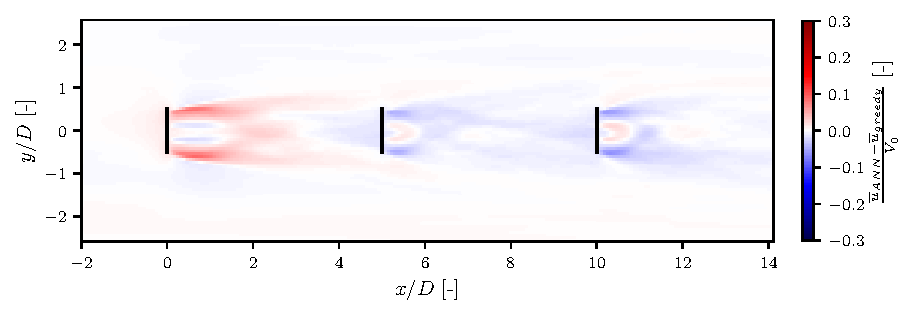
\includegraphics{plots/behaviour_optimization/torque_short_low_velocity_difference.pdf}
	\caption{{\color{black} \rule[3pt]{22pt}{1pt} Turbine.} Mean wake deficit of the ANN-controller compared to the mean wake deficit of a greedy-controlled park.}
	\label{fig:torque_vel_diff}
\end{figure} \\
The difference in mean wake deficit of the ANN controller to the greedy controller is shown in \autoref{fig:torque_vel_diff}. While the wake deficit directly behind the first turbine is lower, when the park is controlled by the ANN, it is higher in front of the second turbine and after the second and third turbine. Therefore the mixing of slow fluid in the wake and undisturbed fluid seems to be reduced. However, the increase in the near wake velocity after the first turbine is still of interest if turbines can not be placed as far apart as in this case. In such a case, a slow reacting greedy controller might still offer benefits for increasing power production.
\begin{figure}[h]
	\centering
	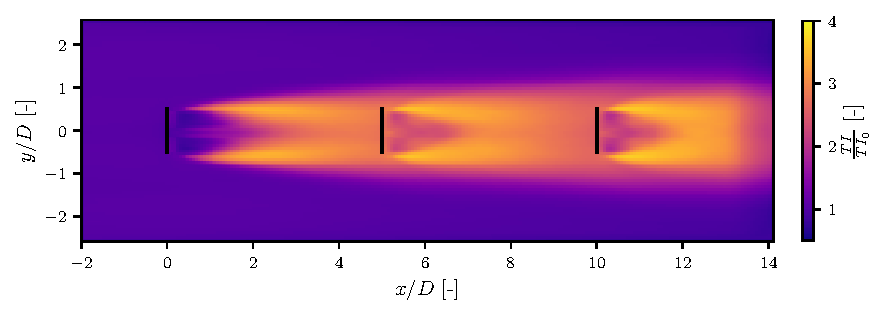
\includegraphics{plots/behaviour_optimization/torque_short_low_turbulence_intensity.pdf}
	\caption{{\color{black} \rule[3pt]{22pt}{1pt} Turbine.} Turbulence intensity of ANN controller compared to turbulence intensity at the inlet.}
	\label{fig:torque_ti}
\end{figure} \\
In \autoref{fig:torque_ti} the turbulence intensity is shown. Here the difference to the helix control becomes very apparent. In the wake of the first turbine the turbulence intensity in the tip vortices of the blades is significantly lower and the wake further down is not as spread out. Instead, the tip vortices hit the blade tips of the second turbine. Overall the turbulence intensity is significantly lower, reducing the mixing of the wake with the undisturbed surrounding fluid. In the second and third wake the turbulence intensity increases and the tip vortices are more spread out. 
\begin{figure}[h]
	\centering
	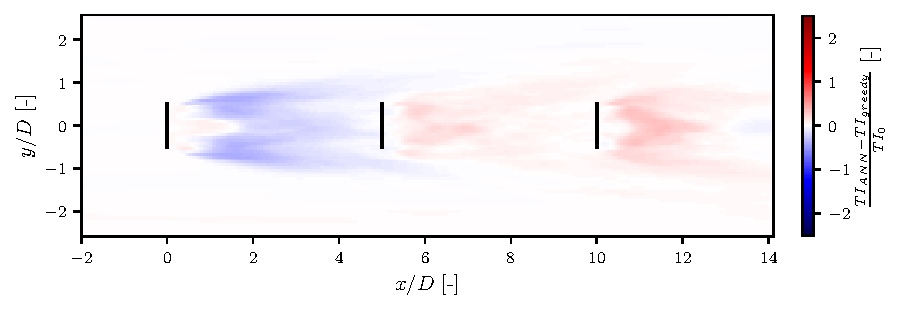
\includegraphics{plots/behaviour_optimization/torque_short_low_ti_difference.pdf}
	\caption{{\color{black} \rule[3pt]{22pt}{1pt} Turbine.} Turbulence intensity of optimized helix control.}
	\label{fig:torque_ti_diff}
\end{figure} \\
Lastly, the difference in turbulence intensity in a park controlled by the ANN controller to a park that is greedy-controlled is shown in \autoref{fig:torque_ti_diff}. The turbulence intensity of the wake after the first turbine is significantly lower in the park controlled by the ANN controller. On the one hand this is probably one of the most important reasons why the wake-mixing is so significantly smaller and therefore power production by the second and third turbine decreased, this might also be a reason for a decrease in fluctuations in power. Therefore, this control strategy of a slow greedy controller might be a possible form improving power quality when parks are de-rated due to overproduction, a scenario that will become more likely in the future, if the total production capacities have increased. In the wake of the second and third turbine turbulence intensity has slightly increased, although the turbulence intensity of the inflow of the third turbine has not changed. \\
Overall the development of a new strategy was not successful. None of the agents were able reach the performance of a greedy controller, despite long training. However, since the coupling of the wind park to the agent worked and the learning algorithm also worked, the problems have to lay in the formulation of the problem, that is, how reward, state and action are connected to the wind park.
\subsubsection{Analysis of the difficulties of training an RL-agent to control a wind park}
Since reinforcement learning has never been applied to an active flow control problem with the properties of this case, namely a fully turbulent flow with multiple actuators separated in space and time, many aspects of this problem have not yet been explored.
As was seen by the comparison of agents trained with different episode lengths, the ratio of episode length to discount factor is very important to the ability to improve behaviour. More general, a high correlation between action and return is necessary for learning. Three possible ways can be identified, how the current formulation of the problem might decrease this correlation.  \\ 
The first can be found by observing the evolution of the control strategy of all three agents trained. While the agents with their initial policy show some reaction to input of the network, that is the velocity probes and the angular velocity of the rotors, this is not visible any more after half of the training time. This can be explained by the fact, that the action set during the beginning of the training is, on average, much lower than the generator torque of the greedy controller for example. Therefore the return does not actually depend on the action, since a higher value of the action is always better than a lower value. Therefore all the weights will eventually be set to zero and only the biases of the last layer will be of any importance. Once that is the case, the influence of the state of the environment has been eliminated and can not come back. Therefore more attention will have to be paid to the translation from the agent's action to the actual generator torque set at the turbine, so that the actions chosen in the beginning are closer to the values necessary for optimal behaviour. Multiple ways to achieve this are possible. One could use an additional layer of nodes with a linear activation function that act as the affine transformation used for non-dimensionalization. However, this would require additional training. Another possible solution is a non-dimensionalization based on mean generator torques used by a greedy controller in preliminary studies. Additionally, the agent could also be trained via supervised learning to behave like a greedy controller before applying reinforcement learning to develop new strategies.\\
The second problem was already identified in \autoref{ssec:new_behaviour_description}. The reward is the total generated power. However, the three different turbines will produce different amounts of power, especially in the beginning of the training. Therefore the first turbine will be improved the fastest, since increasing the efficiency of this turbine yields the greatest gain in reward. The obvious solution would be to either weigh the turbines differently or change the reward to the sum of the power coefficients. However, optimizing power coefficients would result in a greedy strategy, as the greedy control guarantees optimal power coefficient. The same problem arises when using a weighted sum. If the agent would maximize the reward that is a weighted sum of power produced by the different turbines, this would not be the same as maximizing the total power. Thus these two paths can not be the solution. \\
The closer analysis of the reward also revealed another problem already mentioned in \autoref{ssec:new_behaviour_description}. At any moment in time, the power produced by the first turbine only depends on the actions of the agent at the first turbine taken at that moment and in the past. The power of the second turbine depends on the actions of the agent taken at the second turbine at this moment and in the past and on the actions taken by the agent at the first turbine, the time it takes for information to travel from the first turbine to the second turbine ago. The similar argument can be made for the third turbine. Assuming that the influence of an action on the power only lasts for one time step, the return can be phrased the following way:
\begin{equation}
\mathsf{G}_t(\vec{\mathsf{a}}_t, \Gamma) = P_{0,t}(\vec{\mathsf{a}}_t) +P_{1,t+T_{travel}}(\vec{\mathsf{a}}_t) \gamma^{T_{travel}} +P_{2,t+2T_{travel}}(\vec{\mathsf{a}}_t)\gamma^{2T_{travel}} + \Gamma,
\end{equation}
with $\Gamma$ being all other influences. $\Gamma$ is proportional to $\gamma$, since more time steps are included in the calculation of $\mathsf{G}_t$, if $\gamma$ is larger. On the other hand, the weight of the power at the second and third turbine is also directly proportional to $\gamma$. One possible solution to both problems would be the use of independent MDPs, that control one turbine each and have different rewards. Changing the reward of the first environment to 
\begin{equation}
	\mathsf{R}_{0,t} = P_{0,t} +P_{1,t+T_{travel}} +P_{2,t+2T_{travel}}
\end{equation}
would allow for a lower discount rate and eliminate the time shifted influence of actions. The other agents would be seen as part of the environment. Furthermore, this requires no weighting of generated power. However, this would require significant changes to the framework developed for this work and was therefore not implemented. \\